\documentclass[9pt,letterpaper]{article}
\usepackage{pdfpages}
\usepackage{fancyhdr}
\usepackage[colorlinks=true, urlcolor=blue, linkcolor=blue]{hyperref}
\usepackage{graphicx}
\usepackage[top=1.4in, left=0.5in, right=0.9in, bottom=0.8in, landscape]{geometry}
\usepackage{adjustbox}
\usepackage{color, colortbl}
\usepackage[T1]{fontenc}
\usepackage{helvet}
\usepackage{ragged2e}
\pagestyle{fancy}
\renewcommand{\headrulewidth}{0pt}
\renewcommand{\footrulewidth}{0pt}
\setlength{\parindent}{0em}
\setlength{\parskip}{1em}
\definecolor{LightBlue}{rgb}{127,214,246}

\fancyfoot[C]{\setlength{\unitlength}{1in}\begin{picture}(5,0)\put(-3.4,-1){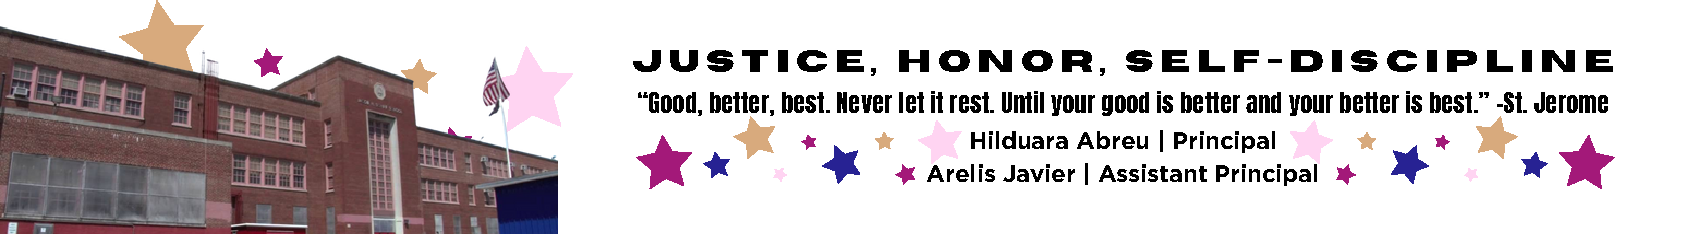
\includegraphics[width=11.9in,height=1.3in]{logo-1}}\end{picture}}
\fancyhead[C]{\setlength{\unitlength}{1in}\begin{picture}(5,0)\put(-3,-0.8){
\includegraphics[width=10.9in,height=1.2in]{logo-2}}\end{picture}}

\pagenumbering{gobble}
\addtolength{\evensidemargin}{-2in}
\addtolength{\topmargin}{-0.5in}
\addtolength{\textwidth}{0in}
%%%%%%%%%%%%%%%%%%%%%%%%%%%%%%%%%%%%%%%%%%%%%%%%%%%%%%%%%%%%%%%%%%

\begin{document}
\vspace*{0.2in}
\textbf{Objetivo: Acuerdo Entre La Escuela y El Hogar, School Academic Year 2024-25}

\begin{tabular}{|p{3.2in}|p{3.2in}|p{3.2in}|}\hline
\Centering{La Escuela:} & \Centering{Los Padres/Guardianes:} & \Centering{Los Alumnos:}\\\hline
	\begin{itemize}
	\item Proporcionar un ambiente seguro y feliz donde todos los niños son
	valorados, respetados y escuchados.
	\item Proporcionar una enseñanza ejemplar y un atractivo plan de estudios
	para satisfacer las necesidades de todos los niños.
	\item Proporcionar oportunidades para que su hijo practique lo que han 
	aprendido en la escuela en casa.
	\item Comparta regularmente el progreso de su hijo y desarrollo a través de
	informes trimestrales y reuniones de padres, “martes fenomenales”.
	\item Ayudar a desarrollar fuertes interacciones sociales y construir 
	autoestima y sentido de la responsabilidad en los niños mediante el 
	establecimiento de altos estándares de comportamiento.
	\item Enseña a tu hijo a desarrollar una actitud positiva hacia los demás,
	independientemente de su sexo, raza, cultura, creencias, valores, edad y/o
	credo.
	\item Proporcionar comunicación sobre la escuela pertinentea reglamentos,
	reuniones, talleres y eventos. Mantendremos nuestro sitio web actualizado,
	enviando boletines informativos con regularidad, y actualizando nuestro 
	calendario de eventos regularmente.
	\end{itemize}
	& 
	\begin{itemize}
	\item Asegurarme de que mi hijo asista a la escuela constantemente y llegue a
	tiempo (8:00 am) usando su uniforme escolar.
	\item Informar a la escuela sobre cualquier inquietud o preocupación que 
	pueda estar afectando el aprendizaje, el comportamiento o la capacidad de mi
	hijo para aprender en casa.
	\item Apoyar a P.S. 192 en su Filosofía de educación basada en valores 
	animando a mi hijo a tener una actitud positiva hacia nuestra comunidad,
	diversa y multicultural.
	\item Asistir a las reuniones con el maestro de mi hijo y otro personal de la
	escuela, con el objetivo de ser positivo y productivo mientras se trabaja 
	para que mi hijo avance en su aprendizaje.
	\item Apoyar y colaborar con la escuela para garantizar que se respeten los 
	reglamentos académicos y de comportamiento.
	\item Leer la información en el sitio web de la escuela, los boletines 
	mensuales, los anuncios semanales y el calendario para estar al tanto de los
	reglamentos, reuniones y eventos relevantes.
	\end{itemize}
 	& 
 	\begin{itemize}
 	\item Asistir a la escuela regularmente, a tiempo y en uniforme.
 	\item Respetar las culturas, razas, sentimientos, creencias y valores de los
 	demás de acuerdo con P.S. 192 y la filosofía de enseñanza basada en valores.
 	\item Respeta nuestras reglas de oro, “Justicia, Honor y Auto-disciplina”
 		\begin{itemize}
 		\item Somos considerados y amables; prestamos mucha atención y somos 
 		responsables de nuestras acciones.
 		\end{itemize}
	\item Ser responsable de mi escuela y el aprendizaje en el hogar.
	\item Cuidar adecuadamente el edificio, el equipo y los predios de la 
	escuela.
	\item Informar a un miembro del personal si estoy preocupado o descontento.
 	\end{itemize}
 \\\hline

\end{tabular}
	

\end{document}
